\subsection{積}\label{chap-4.1-product}
  集合における直積集合を圏に一般化した\textbf{積}を扱う。集合の圏が積の普遍性を持つことは別の章で証明するため、気になった場合は先にそちらを読んでほしい。
	\begin{define}[積]\label{def-product}
		対象$A$と$B$が積を持つとは、以下の条件を満たす組$(A\times B,\pi_{L,A\times B},\pi_{R,A\times B})$が存在するときである。
		\begin{quote}
			\begin{mydescription}
			\item[積対象と射影射]ある対象$A\times B$とある二つの射$\mor{\pi_{L,A\times B}}{A\times B}{A}$、$\mor{\pi_{R,A\times B}}{A\times B}{B}$が存在する。\\
      この時$A\times B$を\textbf{積対象}と呼び、$\pi_{L,A\times B},\ \pi_{R,A\times B}$を\textbf{射影射}と呼ぶことにする。また正確に記述したい場合、積対象と射影射の組$(A\times B,\pi_{L,A\times B},\pi_{R,A\times B})$を$A,B$の\textbf{積}と呼ぶことにする。

			\begin{center}
				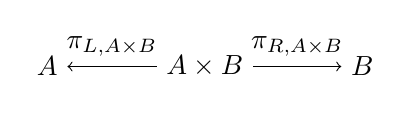
\begin{tikzpicture}[auto]
					\node (a) at (0, 0) {$A$};
					\node (b) at (4, 0) {$B$};
					\node (ab) at (2, 0) {$A\times B$};
					\draw[->] (ab) to node[swap] {$\pi_{L,A\times B}$}(a);
					\draw[->] (ab) to node {$\pi_{R,A\times B}$}(b);
				\end{tikzpicture}
			\end{center}
			また$(A\times A,\pi_{L,A\times B},\pi_{R,A\times B})$などの紛らわしい場合を除いて$\pi_{L,A\times B}$を$\pi_A$、$\pi_{R,A\times B}$を$\pi_B$と表記する。
			\item[任意の対象からの射]任意の対象$X$に対し任意の二射$\mor{f}{X}{A}$、$\mor{g}{X}{B}$が存在するとする。
			\begin{center}
				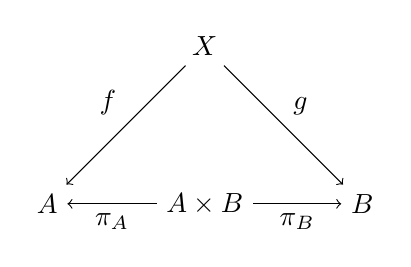
\begin{tikzpicture}[auto]
					\node (a) at (0, 0) {$A$};
					\node (b) at (4, 0) {$B$};
					\node (ab) at (2, 0) {$A\times B$};
					\node (x) at (2, 2) {$X$};
					\draw[->] (ab) to node {$\pi_A$}(a);
					\draw[->] (ab) to node[swap] {$\pi_B$}(b);
					\draw[->] (x) to node[swap] {$f$}(a);
					\draw[->] (x) to node {$g$}(b);
				\end{tikzpicture}
			\end{center}
			\item[普遍性]任意の二射$f,g$に対して図式を可換にする、つまり\[\pi_A\circ t=f,\ \pi_B\circ t=g\]が成り立つような射$t$が少なくとも一つは存在し、このような$t$を$\tuple{f,g}$と表記する。\\
      この時、$\tuple{f,g}$を$f,g$に対する\textbf{射の対}と呼ぶことにする。
			また射の対$\tuple{f,g}$は任意の二射$f,g$に対して\textbf{一意}に\textbf{存在}する。\\
      ここでの射の対が一意であるとは、ある射$\mor{t}{X}{A\times B}$が\[\pi_A\circ t=f,\ \pi_B\circ t=g\]を満たす。すなわち射の対であるとき、同様にある射$\mor{h}{X}{A\times B}$も同様に\[\pi_A\circ h=f,\ \pi_B\circ h=g\]を満たし射の対であるとき、$h=t=\tuple{f,g}$が成り立つということである。\\
			\begin{center}
				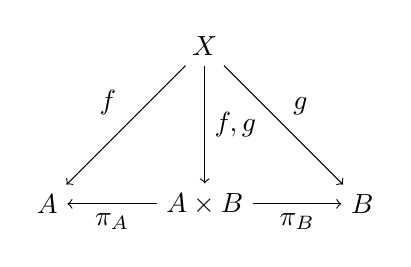
\begin{tikzpicture}[auto]
					\node (a) at (0, 0) {$A$};
					\node (b) at (4, 0) {$B$};
					\node (ab) at (2, 0) {$A\times B$};
					\node (x) at (2, 2) {$X$};
					\draw[->] (ab) to node {$\pi_A$}(a);
					\draw[->] (ab) to node[swap] {$\pi_B$}(b);
					\draw[->] (x) to node[swap] {$f$}(a);
					\draw[->] (x) to node {$g$}(b);
					\draw[->] (x) to node {$\tuple{f,g}$}(ab);
				\end{tikzpicture}
			\end{center}
			\end{mydescription}
		\end{quote}

	\end{define}
	また、図式を可換にする射の対$\tuple{f,g}$の存在性は任意の射の組み合わせに対して射の対が存在することを示し、一意性は射の対が含んでいる二つの射以外の判別可能な要素を含みようがないことを示している。

	\begin{define}[積を持つ圏]\label{def-category-with-product}
		すべての圏、すべての二対象に対して積が存在するとは限らないが、ある圏$\cat{C}$の任意の二対象に対して積が存在するとき、圏$\cat{C}$は\textbf{積を持つ}という。
	\end{define}
	ここで$X$に終対象$1$を当てはめると、元$\mor{a}{1}{A}$、元$\mor{b}{1}{B}$に対して$\pi_A\circ\tuple{a,b}=a$、$\pi_B\circ\tuple{a,b}=b$が成り立つような$\tuple{a,b}$が一意に存在することがわかる。
	\begin{center}
		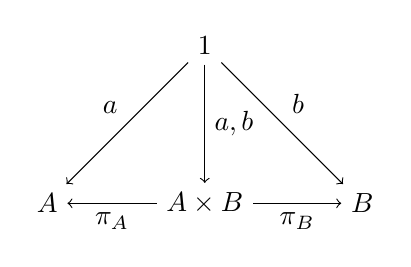
\begin{tikzpicture}[auto]
			\node (a) at (0, 0) {$A$};
			\node (b) at (4, 0) {$B$};
			\node (ab) at (2, 0) {$A\times B$};
			\node (x) at (2, 2) {$1$};
			\draw[->] (ab) to node {$\pi_A$}(a);
			\draw[->] (ab) to node[swap] {$\pi_B$}(b);
			\draw[->] (x) to node[swap] {$a$}(a);
			\draw[->] (x) to node {$b$}(b);
			\draw[->] (x) to node {$\tuple{a,b}$}(ab);
		\end{tikzpicture}
	\end{center}

	次に積の普遍性を用いた証明の練習として、射の対が合成に対して分配的であることを示そう。
	\begin{prop}[射の対の分配則]\label{prop-distributive-law-at-pair-of-arrows}
		$\mor{f}{X}{A}$、$\mor{g}{X}{B}$、$\mor{h}{Y}{X}$に対して\[\tuple{f,g}\circ h=\tuple{f\circ h,g\circ h}\]が成り立つ
	\end{prop}
	\begin{proof}
		積$A\times B$に対し、$\mor{f\circ h}{Y}{A}$、$\mor{g\circ h}{Y}{B}$の射の対$\mor{\tuple{f\circ h,g\circ h}}{Y}{A\times B}$を考える。

		これは$\mor{\tuple{f,g}\circ h}{Y}{A\times B}$が二射$f\circ h,g\circ h$における射の対となることを示し、射の対の一意性から証明すればよい。

		積の普遍性より、
		\begin{align*}
			\pi_A\circ\tuple{f\circ h,g\circ h}&=f\circ h\\
			\pi_B\circ\tuple{f\circ h,g\circ h}&=g\circ h
		\end{align*}
		が成り立つような射$\tuple{f\circ h,g\circ h}$は一意に存在する。

		また、
		\begin{align*}
			\pi_A\circ(\tuple{f,g}\circ h)&=(\pi_A\circ\tuple{f,g})\circ h&\text{(結合則)}\\
			&=f\circ h&\text{(射の対の可換性)}\\
			\pi_B\circ(\tuple{f,g}\circ h)&=(\pi_B\circ\tuple{f,g})\circ h&\text{(結合則)}\\
			&=g\circ h&\text{(射の対の可換性)}
		\end{align*}
		$\pi_A\circ(\tuple{f,g}\circ h)=f\circ h$、$\pi_B\circ(\tuple{f,g}\circ h)=g\circ h$となるため、$\mor{\tuple{f,g}\circ h}{Y}{A\times B}$も同様に二射$f\circ h,g\circ h$の射の対になる。
		よって射の対の一意性より、$\tuple{f,g}\circ h=\tuple{f\circ h,g\circ h}$が成り立つ。
	\end{proof}

	\begin{center}
		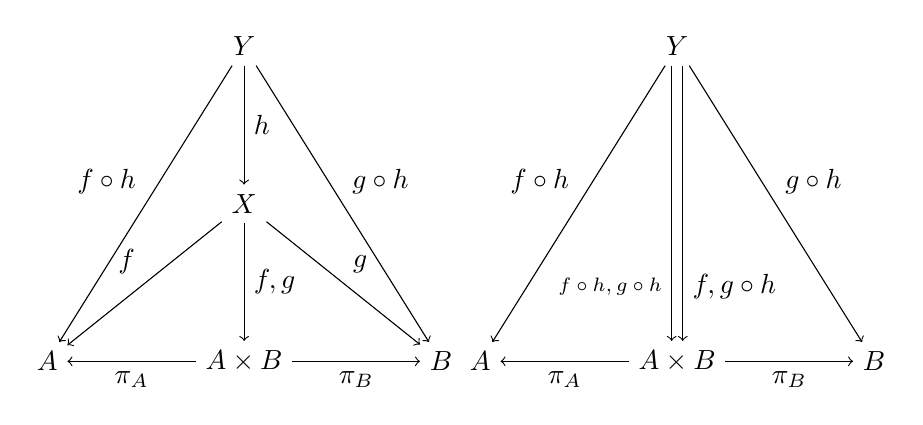
\begin{tikzpicture}[auto]
			\node (y) at (3, 4) {$Y$};
			\node (a) at (0.5, 0) {$A$};
			\node (b) at (5.5, 0) {$B$};
			\node (ab) at (3, 0) {$A\times B$};
			\node (x) at (3, 2) {$X$};
			\draw[->] (y) to node {$h$}(x);
			\draw[->] (y) to node[swap] {$f\circ h$}(a);
			\draw[->] (y) to node {$g\circ h$}(b);
			\draw[->] (ab) to node {$\pi_A$}(a);
			\draw[->] (ab) to node[swap] {$\pi_B$}(b);
			\draw[->] (x) to node[swap] {$f$}(a);
			\draw[->] (x) to node {$g$}(b);
			\draw[->] (x) to node {$\tuple{f,g}$}(ab);

			\node (y) at (8.5, 4) {$Y$};
			\node (a) at (6, 0) {$A$};
			\node (b) at (11, 0) {$B$};
			\node (ab) at (8.5, 0) {$A\times B$};
			\draw[->, transform canvas={xshift=2pt}] (y) to node[yshift=-30pt] {$\tuple{f,g}\circ h$}(ab);
			\draw[->, transform canvas={xshift=-2pt}] (y) to node[yshift=-30pt, swap] {\scriptsize{$\tuple{f\circ h,g\circ h}$}}(ab);
			\draw[->] (y) to node[swap] {$f\circ h$}(a);
			\draw[->] (y) to node {$g\circ h$}(b);
			\draw[->] (ab) to node {$\pi_A$}(a);
			\draw[->] (ab) to node[swap] {$\pi_B$}(b);
		\end{tikzpicture}
	\end{center}

  普遍性を用いた基本的な等式の証明はこのように、等式の右辺左辺が同じ二射の射の対になるような図式を考え、射の対の一意性から等式を示す。
  この証明では積の図式に対象$Y$と射$h$をつなげて拡張することで、新しい積の図式を考えた。

	また$Y$に終対象$1$、$h$に元$\mor{x}{1}{X}$を当てはめると、同様に$\tuple{f,g}\circ x=\tuple{f\circ x,g\circ x}$となる。
	つまり射の対は与えられた元にそれぞれの射を適用し、また対を取るような射だと考えられる。
	\begin{center}
		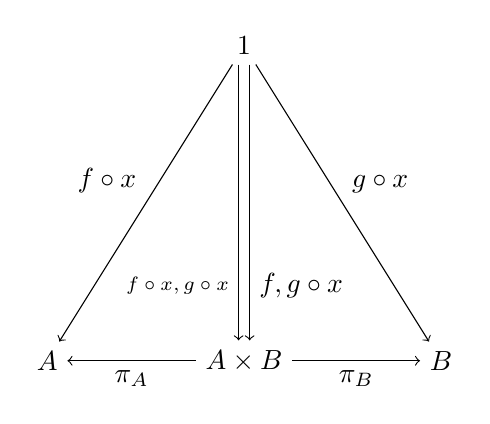
\begin{tikzpicture}[auto]
			\node (y) at (8.5, 4) {$1$};
			\node (a) at (6, 0) {$A$};
			\node (b) at (11, 0) {$B$};
			\node (ab) at (8.5, 0) {$A\times B$};
			\draw[->, transform canvas={xshift=2pt}] (y) to node[yshift=-30pt] {$\tuple{f,g}\circ x$}(ab);
			\draw[->, transform canvas={xshift=-2pt}] (y) to node[yshift=-30pt, swap] {\scriptsize{$\tuple{f\circ x,g\circ x}$}}(ab);
			\draw[->] (y) to node[swap] {$f\circ x$}(a);
			\draw[->] (y) to node {$g\circ x$}(b);
			\draw[->] (ab) to node {$\pi_A$}(a);
			\draw[->] (ab) to node[swap] {$\pi_B$}(b);
		\end{tikzpicture}
	\end{center}

	次に任意の積から任意の積への射である、射の積を定義していく。
	\begin{define}[射の積]\label{def-product-of-arrows}
		射$\mor{f}{A}{A'}$、$\mor{g}{B}{B'}$に対して射の積$\mor{f\times g}{A\times B}{A'\times B'}$を\[f\times g = \tuple{f\circ\pi_A,g\circ\pi_B}\]と定義する。
		\begin{center}
			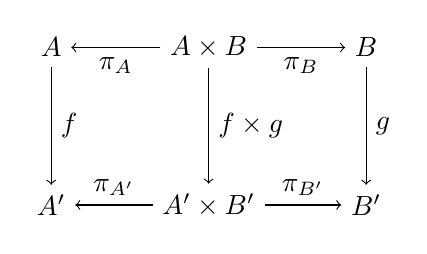
\begin{tikzpicture}[auto]
				\node (a) at (0, 0) {$A$};
				\node (ab) at (2, 0) {$A\times B$};
				\node (b) at (4, 0) {$B$};
				\node (a') at (0, -2) {$A'$};
				\node (a'b') at (2, -2) {$A'\times B'$};
				\node (b') at (4, -2) {$B'$};
				\draw[->] (a'b') to node[swap] {$\pi_{A'}$}(a');
				\draw[->] (a'b') to node {$\pi_{B'}$}(b');
				\draw[->] (ab) to node {$\pi_A$}(a);
				\draw[->] (ab) to node[swap] {$\pi_B$}(b);
				\draw[->] (a) to node {$f$}(a');
				\draw[->] (b) to node {$g$}(b');
				\draw[->] (ab) to node {$f\times g$}(a'b');
			\end{tikzpicture}
		\end{center}
	\end{define}
	射の対は任意の対象から任意の積への射であるのに対し、射の積は任意の積から任意の積への射である。
	二つの対象から二つの対象へ射を一つの射に纏めることから、直感的に射の積は並列処理のように思える。

	\begin{prop}[積と合成の交換]\label{prop-commutativity-of-product-and-composition}
		射の積$\mor{f\times g}{A\times B}{A'\times B'}$、$\mor{f'\times g'}{A'\times B'}{A''\times B''}$に対して、\[(f'\times g')\circ(f\times g)=(f'\circ f)\times(g'\circ g)\]が成り立つ。
	\end{prop}
	\begin{proof}
		積$(A''\times B'',\pi_{A''},\pi_{B''})$において対$(X,f,g)$に$(A\times B,f'\circ f\circ\pi_A$,$g'\circ g\circ\pi_B)$を当てはめると射$\mor{\tuple{f'\circ f\circ\pi_A,g'\circ g\circ\pi_B}}{A\times B}{A''\times B''}$が得られる。また射の積の定義より\[\tuple{f'\circ f\circ\pi_A,g'\circ g\circ\pi_B}=(f'\circ f)\times(g'\circ g)\]が成り立つ。
		次に$(f'\times g')\circ(f\times g)$も同様に$(A\times B,f'\circ f\circ\pi_A$,$g'\circ g\circ\pi_B)$に対する射の対であることを示す。
		\begin{align*}
			\pi_{A''}\circ(f'\times g')\circ(f\times g)&=\pi_{A''}\circ\tuple{f'\circ\pi_A,g'\circ\pi_B}\circ\tuple{f\circ\pi_A,g\circ\pi_B}&\text{(射の積の定義)}\\
			&=f'\circ\pi_{A'}\circ\tuple{f\circ\pi_A,g\circ\pi_B}&\text{(射の対の可換性)}\\
			&=f'\circ f\circ\pi_A&\text{(射の対の可換性)}\\
			\pi_B\circ(f'\times g')\circ(f\times g)&=\pi_{B''}\circ\tuple{f'\circ\pi_A,g'\circ\pi_B}\circ\tuple{f\circ\pi_A,g\circ\pi_B}&\text{(射の積の定義)}\\
			&=g'\circ\pi_{B'}\circ\tuple{f\circ\pi_A,g\circ\pi_B}&\text{(射の対の可換性)}\\
			&=g'\circ g\circ\pi_B&\text{(射の対の可換性)}
		\end{align*}
	\begin{center}
		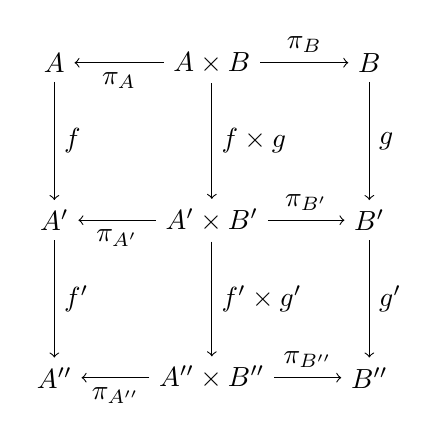
\begin{tikzpicture}[auto]
			\node (a) at (0, 0) {$A$};
			\node (a') at (0, -2) {$A'$};
			\node (a'') at (0, -4) {$A''$};
			\node (ab) at (2, 0) {$A\times B$};
			\node (ab') at (2, -2) {$A'\times B'$};
			\node (ab'') at (2, -4) {$A''\times B''$};
			\node (b) at (4, 0) {$B$};
			\node (b') at (4, -2) {$B'$};
			\node (b'') at (4, -4) {$B''$};
			\draw[->] (ab) to node{$\pi_{A}$}(a);
			\draw[->] (ab) to node{$\pi_{B}$}(b);
			\draw[->] (ab') to node{$\pi_{A'}$}(a');
			\draw[->] (ab') to node{$\pi_{B'}$}(b');
			\draw[->] (ab'') to node{$\pi_{A''}$}(a'');
			\draw[->] (ab'') to node{$\pi_{B''}$}(b'');
			\draw[->] (a) to node{$f$}(a');
			\draw[->] (a') to node{$f'$}(a'');
			\draw[->] (b) to node{$g$}(b');
			\draw[->] (b') to node{$g'$}(b'');
			\draw[->] (ab) to node{$f\times g$}(ab');
			\draw[->] (ab') to node{$f'\times g'$}(ab'');
		\end{tikzpicture}
		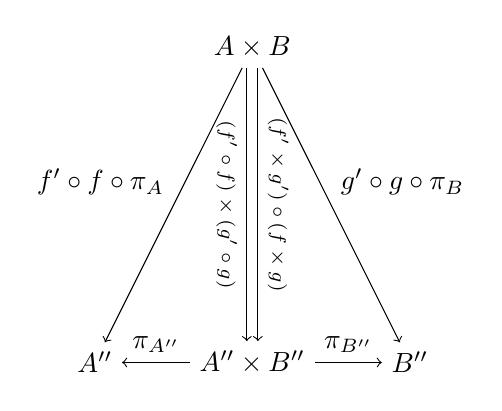
\begin{tikzpicture}[auto]
			\node (a'') at (0, -4) {$A''$};
			\node (ab) at (2, 0) {$A\times B$};
			\node (ab'') at (2, -4) {$A''\times B''$};
			\node (b'') at (4, -4) {$B''$};
			\draw[->] (ab) to node[swap]{$f'\circ f\circ\pi_A$}(a'');
			\draw[->] (ab) to node{$g'\circ g\circ\pi_B$}(b'');
			\draw[->] (ab'') to node[swap]{$\pi_{A''}$}(a'');
			\draw[->] (ab'') to node{$\pi_{B''}$}(b'');
			\draw[->,transform canvas={xshift=2pt}] (ab) to node[sloped]{\scriptsize{$(f'\times g')\circ(f\times g)$}} (ab'');
			\draw[->,transform canvas={xshift=-2pt}] (ab) to node[sloped,swap]{\scriptsize{$(f'\circ f)\times(g'\circ g)$}}(ab'');
		\end{tikzpicture}
	\end{center}

		\[\pi_A\circ(f'\times g')\circ(f\times g)=f'\circ f\circ\pi_A,\ \pi_B\circ(f'\times g')\circ(f\times g)=g'\circ g\circ\pi_B\]の二式が成り立つから、$(f'\times g')\circ(f\times g)$も同様に$(A\times B,f'\circ f\circ\pi_A$,$g'\circ g\circ\pi_B)$に対する射の対である。

		よって$(f'\times g')\circ(f\times g)=(f'\circ f)\times(g'\circ g)$が成り立つ。
	\end{proof}
	射の積を並列での合成とみなすならば、射の合成は直列での合成を表し、積と合成の交換はどちらの合成を先に計算しても結果が変わらないことを表す。
	\begin{prop}[射影射の対]\label{prop-pair-of-projection}
		ある積$(A\times B,\pi_A,\pi_B)$に対して$\tuple{\pi_A,\pi_B}=id_{A\times B}$が成り立つ。
	\end{prop}
	\begin{proof}
		積$(A\times B,\pi_A,\pi_B)$に対して二射$\pi_A,\pi_B$の射の対$\mor{\tuple{\pi_A,\pi_B}}{A\times B}{A\times B}$を考える。この時、$\mor{id_{A\times B}}{A\times B}{A\times B}$も同様に二射$\pi_A,\pi_B$の射の対であることを示せばよい。


		$\pi_{A}\circ id_{A\times B}=\pi_{A}$と$\pi_{B}\circ id_{A\times B}=\pi_{B}$が成り立つから、$id_{A\times B}$は$\pi_A$と$\pi_B$の射の対になる。よって射の対の一意性より、$\tuple{\pi_A,\pi_B}=id_{A\times B}$が成り立つ。
		\begin{center}
			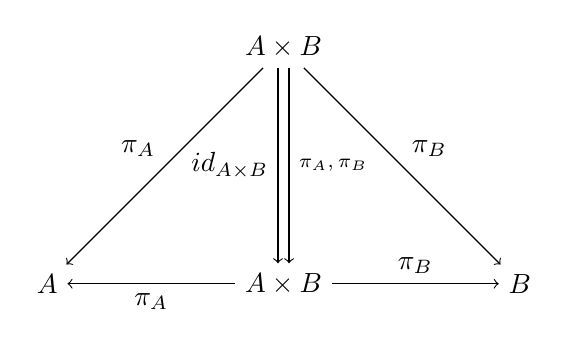
\begin{tikzpicture}[auto]
				\node (a) at (0, 0) {$A$};
				\node (ab) at (3, 0) {$A\times B$};
				\node (b) at (6, 0) {$B$};
				\node (p) at (3, 3) {$A\times B$};
				\draw[->] (p) to node[swap]{$\pi_A$}(a);
				\draw[->] (p) to node{$\pi_B$}(b);
				\draw[->,transform canvas={xshift=2pt}] (p) to node{\scriptsize{$\tuple{\pi_A,\pi_B}$}}(ab);
				\draw[->,transform canvas={xshift=-2pt}] (p) to node[swap]{$id_{A\times B}$}(ab);
				\draw[->] (ab) to node{$\pi_A$}(a);
				\draw[->] (ab) to node{$\pi_B$}(b);
			\end{tikzpicture}
		\end{center}
	\end{proof}
	\begin{prop}[積の一意性]\label{prop-uniqueness-of-products}
		$A$と$B$の積$A\times B$に対して、同様に$A$と$B$の積である対象$P$と射影射$\mor{\rho_A}{P}{A}$、$\mor{\rho_B}{P}{B}$が存在するとき、$A\times B\cong P$が成り立つ。またこの時、積は\textbf{同型を除いて一意}と呼ぶことがある。
	\end{prop}
	\begin{proof}
		対象$A$、$B$の積$(A\times B,\pi_A,\pi_B)$、$(P,\rho_A,\rho_B)$の二つの積を考える必要があるが、ややこしいので少し性質を整理する。
		\begin{quote}
			\begin{mydescription}
				\item[積$(A\times B,\pi_A,\pi_B)$の性質]
				積$A\times B$と射影射$\mor{\pi_A}{A\times B}{A}$、$\mor{\pi_B}{A\times B}{B}$において二つの射$\mor{f}{X}{A}$、$\mor{g}{X}{B}$に対する射の対を$\mor{\tuple{f,g}}{X}{A\times B}$とする。また射$\tuple{f,g}$が積$A\times B$における射の対であるとき、
				\begin{align*}
					\pi_A\circ\tuple{f,g}&=f\\
					\pi_B\circ\tuple{f,g}&=g
				\end{align*}
				が成り立つ。
				またこのような射の対は一意に存在する。
				\begin{center}
					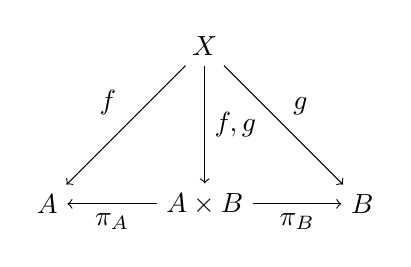
\begin{tikzpicture}[auto]
						\node (a) at (0, 0) {$A$};
						\node (b) at (4, 0) {$B$};
						\node (ab) at (2, 0) {$A\times B$};
						\node (x) at (2, 2) {$X$};
						\draw[->] (ab) to node {$\pi_A$}(a);
						\draw[->] (ab) to node[swap] {$\pi_B$}(b);
						\draw[->] (x) to node[swap] {$f$}(a);
						\draw[->] (x) to node {$g$}(b);
						\draw[->] (x) to node {$\tuple{f,g}$}(ab);
					\end{tikzpicture}
				\end{center}
				\item[積$(P,\rho_A,\rho_B)$の性質]
				積$P$と射影射$\mor{\rho_A}{P}{A}$、$\mor{\rho_B}{P}{B}$において二つの射$\mor{f}{X}{A}$、$\mor{g}{X}{B}$に対する射の対を$\mor{[f,g]}{X}{P}$とする。また射$[f,g]$が積$P$における射の対であるとき、
				\begin{align*}
					\rho_A\circ[f,g]&=f\\
					\rho_B\circ[f,g]&=g
				\end{align*}
				が成り立つ。
				またこのような射の対は一意に存在する。
				\begin{center}
					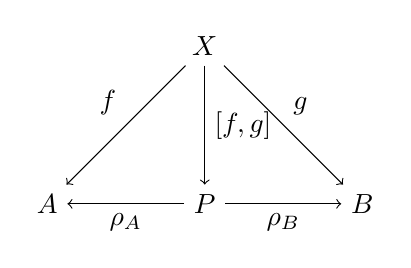
\begin{tikzpicture}[auto]
						\node (a) at (0, 0) {$A$};
						\node (b) at (4, 0) {$B$};
						\node (ab) at (2, 0) {$P$};
						\node (x) at (2, 2) {$X$};
						\draw[->] (ab) to node {$\rho_A$}(a);
						\draw[->] (ab) to node[swap] {$\rho_B$}(b);
						\draw[->] (x) to node[swap] {$f$}(a);
						\draw[->] (x) to node {$g$}(b);
						\draw[->] (x) to node {$[f,g]$}(ab);
					\end{tikzpicture}
				\end{center}
			\end{mydescription}

			積$A\times B$における射の対$\mor{\tuple{f,g}}{X}{A\times B}$に対し、積$P$における射の対$\mor{[f,g]}{X}{P}$は全く別の射である。そのため対の表記で区別することにする。

			また$\pi_A\circ[f,g]=f$は成り立たないどころか、始域、終域は$\mor{\pi_A}{A\times B}{A}$と$\mor{[f,g]}{X}{P}$となり合成すらできないということに注意してほしい。
		\end{quote}
		証明に戻ると、\[[\pi_A,\pi_B]\circ\tuple{\rho_A,\rho_B}=id_P\]と
		\[\tuple{\rho_A,\rho_B}\circ[\pi_A,\pi_B]=id_{A\times B}\]が成り立つことを二つの積の普遍性による射の一意性から示せばよい。具体的にはこれらの射がある積の図式における射の対になることを示し、射の対の一意性から等式を導く。

		積$(A\times B,\pi_A,\pi_B)$において、二射$\rho_A,\rho_B$に対する射の対を\[\mor{\tuple{\rho_A,\rho_B}}{P}{A\times B}\]とする。

		逆に積$(P,\rho_A,\rho_B)$において二射$\pi_A,\pi_B$に対する射の対を\[\mor{[\pi_A,\pi_B]}{A\times B}{P}\]とする。
		\begin{center}
			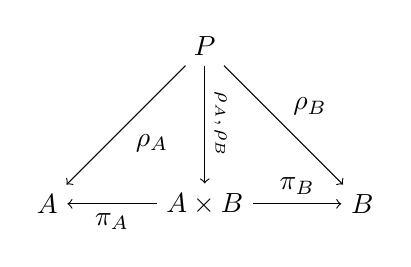
\begin{tikzpicture}[auto]
				\node (a) at (0, 0) {$A$};
				\node (ab) at (2, 0) {$A\times B$};
				\node (b) at (4, 0) {$B$};
				\node (p) at (2, 2) {$P$};
				\draw[->] (p) to node{$\rho_A$}(a);
				\draw[->] (p) to node{$\rho_B$}(b);
				\draw[->] (p) to node[sloped]{\scriptsize{$\tuple{\rho_A,\rho_B}$}}(ab);
				\draw[->] (ab) to node{$\pi_A$}(a);
				\draw[->] (ab) to node{$\pi_B$}(b);
			\end{tikzpicture}
			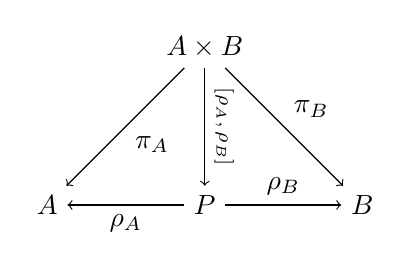
\begin{tikzpicture}[auto]
				\node (a) at (0, 0) {$A$};
				\node (ab) at (2, 2) {$A\times B$};
				\node (b) at (4, 0) {$B$};
				\node (p) at (2, 0) {$P$};
				\draw[->] (p) to node{$\rho_A$}(a);
				\draw[->] (p) to node{$\rho_B$}(b);
				\draw[->] (ab) to node[sloped]{\scriptsize{$[\rho_A,\rho_B]$}}(p);
				\draw[->] (ab) to node{$\pi_A$}(a);
				\draw[->] (ab) to node{$\pi_B$}(b);
			\end{tikzpicture}
		\end{center}
		次に$\mor{\tuple{\rho_A,\rho_B}\circ[\pi_A,\pi_B]}{A\times B}{A\times B}$が$\pi_A$と$\pi_B$の射の対であることを示す。
		\begin{align*}
			\pi_A\circ\tuple{\rho_A,\rho_B}\circ[\pi_A,\pi_B]&=\rho_A\circ[\pi_A,\pi_B]&\text{(積$A\times B$の射の対の可換性)}\\
			&=\pi_A&\text{(積$P$の射の対の可換性)}\\
			\pi_B\circ\tuple{\rho_A,\rho_B}\circ[\pi_A,\pi_B]&=\rho_B\circ[\pi_A,\pi_B]&\text{(積$A\times B$の射の対の可換性)}\\
			&=\pi_B&\text{(積$P$の射の対の可換性)}\\
		\end{align*}
		よって\[\pi_A\circ(\tuple{\rho_A,\rho_B}\circ[\pi_A,\pi_B])=\pi_A,\ \pi_B\circ(\tuple{\rho_A,\rho_B}\circ[\pi_A,\pi_B])=\pi_B\]が成り立つから、$\tuple{\rho_A,\rho_B}\circ[\pi_A,\pi_B]$は射$\pi_A$と$\pi_B$の射の対となる。すると射の対の一意性より、\[\tuple{\rho_A,\rho_B}\circ[\pi_A,\pi_B]=\tuple{\pi_A,\pi_B}=id_{A\times B}\]が成り立つ。
		\begin{center}
			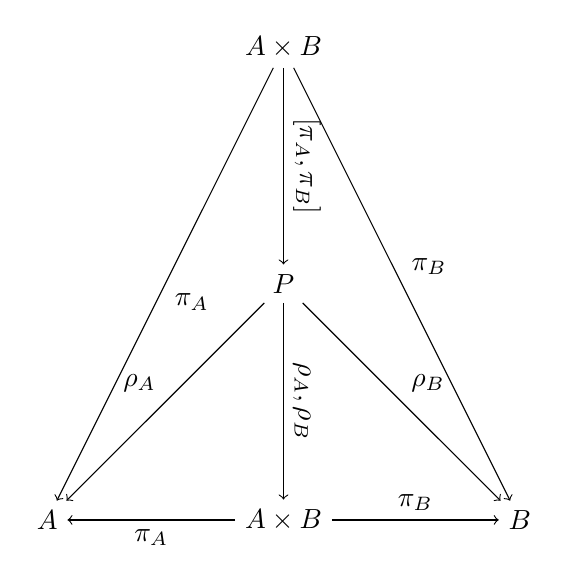
\begin{tikzpicture}[auto]
				\node (a) at (0, 0) {$A$};
				\node (ab) at (3, 0) {$A\times B$};
				\node (ab2) at (3, 6) {$A\times B$};
				\node (b) at (6, 0) {$B$};
				\node (p) at (3, 3) {$P$};
				\draw[->] (p) to node[swap]{$\rho_A$}(a);
				\draw[->] (p) to node{$\rho_B$}(b);
				\draw[->] (p) to node[sloped]{$\tuple{\rho_A,\rho_B}$}(ab);
				\draw[->] (ab2) to node[sloped]{$[\pi_A,\pi_B]$}(p);
				\draw[->] (ab) to node{$\pi_A$}(a);
				\draw[->] (ab) to node{$\pi_B$}(b);
				\draw[->] (ab2) to node{$\pi_A$}(a);
				\draw[->] (ab2) to node{$\pi_B$}(b);
			\end{tikzpicture}
			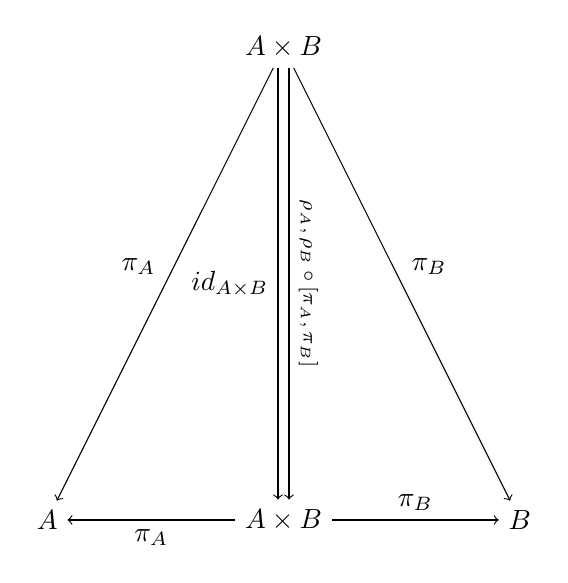
\begin{tikzpicture}[auto]
				\node (a) at (0, 0) {$A$};
				\node (ab) at (3, 0) {$A\times B$};
				\node (b) at (6, 0) {$B$};
				\node (ab2) at (3, 6) {$A\times B$};
				\draw[->] (ab2) to node[swap]{$\pi_A$}(a);
				\draw[->] (ab2) to node{$\pi_B$}(b);
				\draw[->,transform canvas={xshift=2pt}] (ab2) to node[sloped]{\scriptsize{$\tuple{\rho_A,\rho_B}\circ[\pi_A,\pi_B]$}}(ab);
				\draw[->,transform canvas={xshift=-2pt}] (ab2) to node[swap]{$id_{A\times B}$}(ab);
				\draw[->] (ab) to node{$\pi_A$}(a);
				\draw[->] (ab) to node{$\pi_B$}(b);
			\end{tikzpicture}
		\end{center}
		同様に$[\pi_A,\pi_B]\circ\tuple{\rho_A,\rho_B}=id_P$が成り立つから、$[\pi_A,\pi_B]$と$\tuple{\rho_A,\rho_B}$は同型射となり、$A\times B\cong P$が成り立つ。
	\end{proof}
